\subsection{Диаграмма последовательности}
\begin{figure}[H]
	\centering
	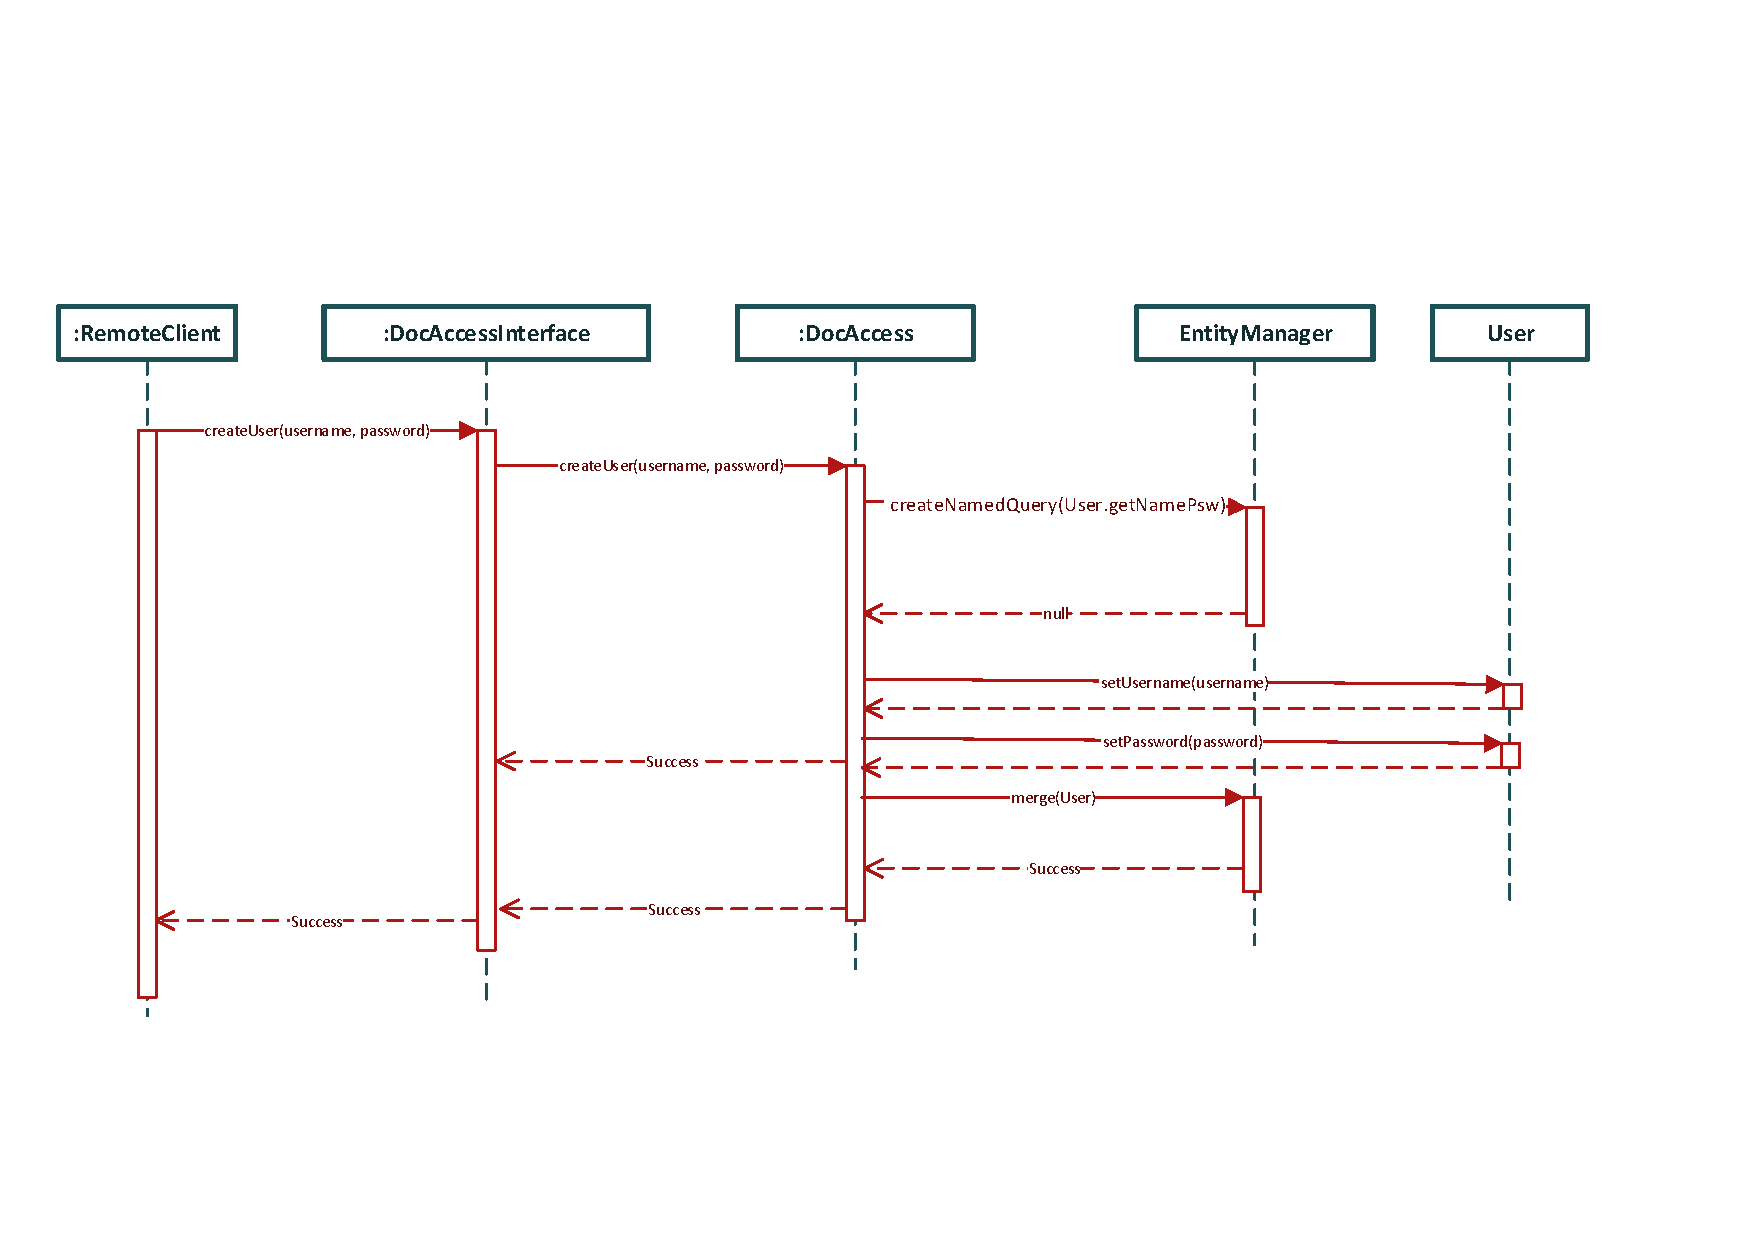
\includegraphics[width=1\textwidth]{createUser}
	\caption{Регистрация}
	\label{fig:reg}
\end{figure}

\begin{figure}[H]
	\centering
	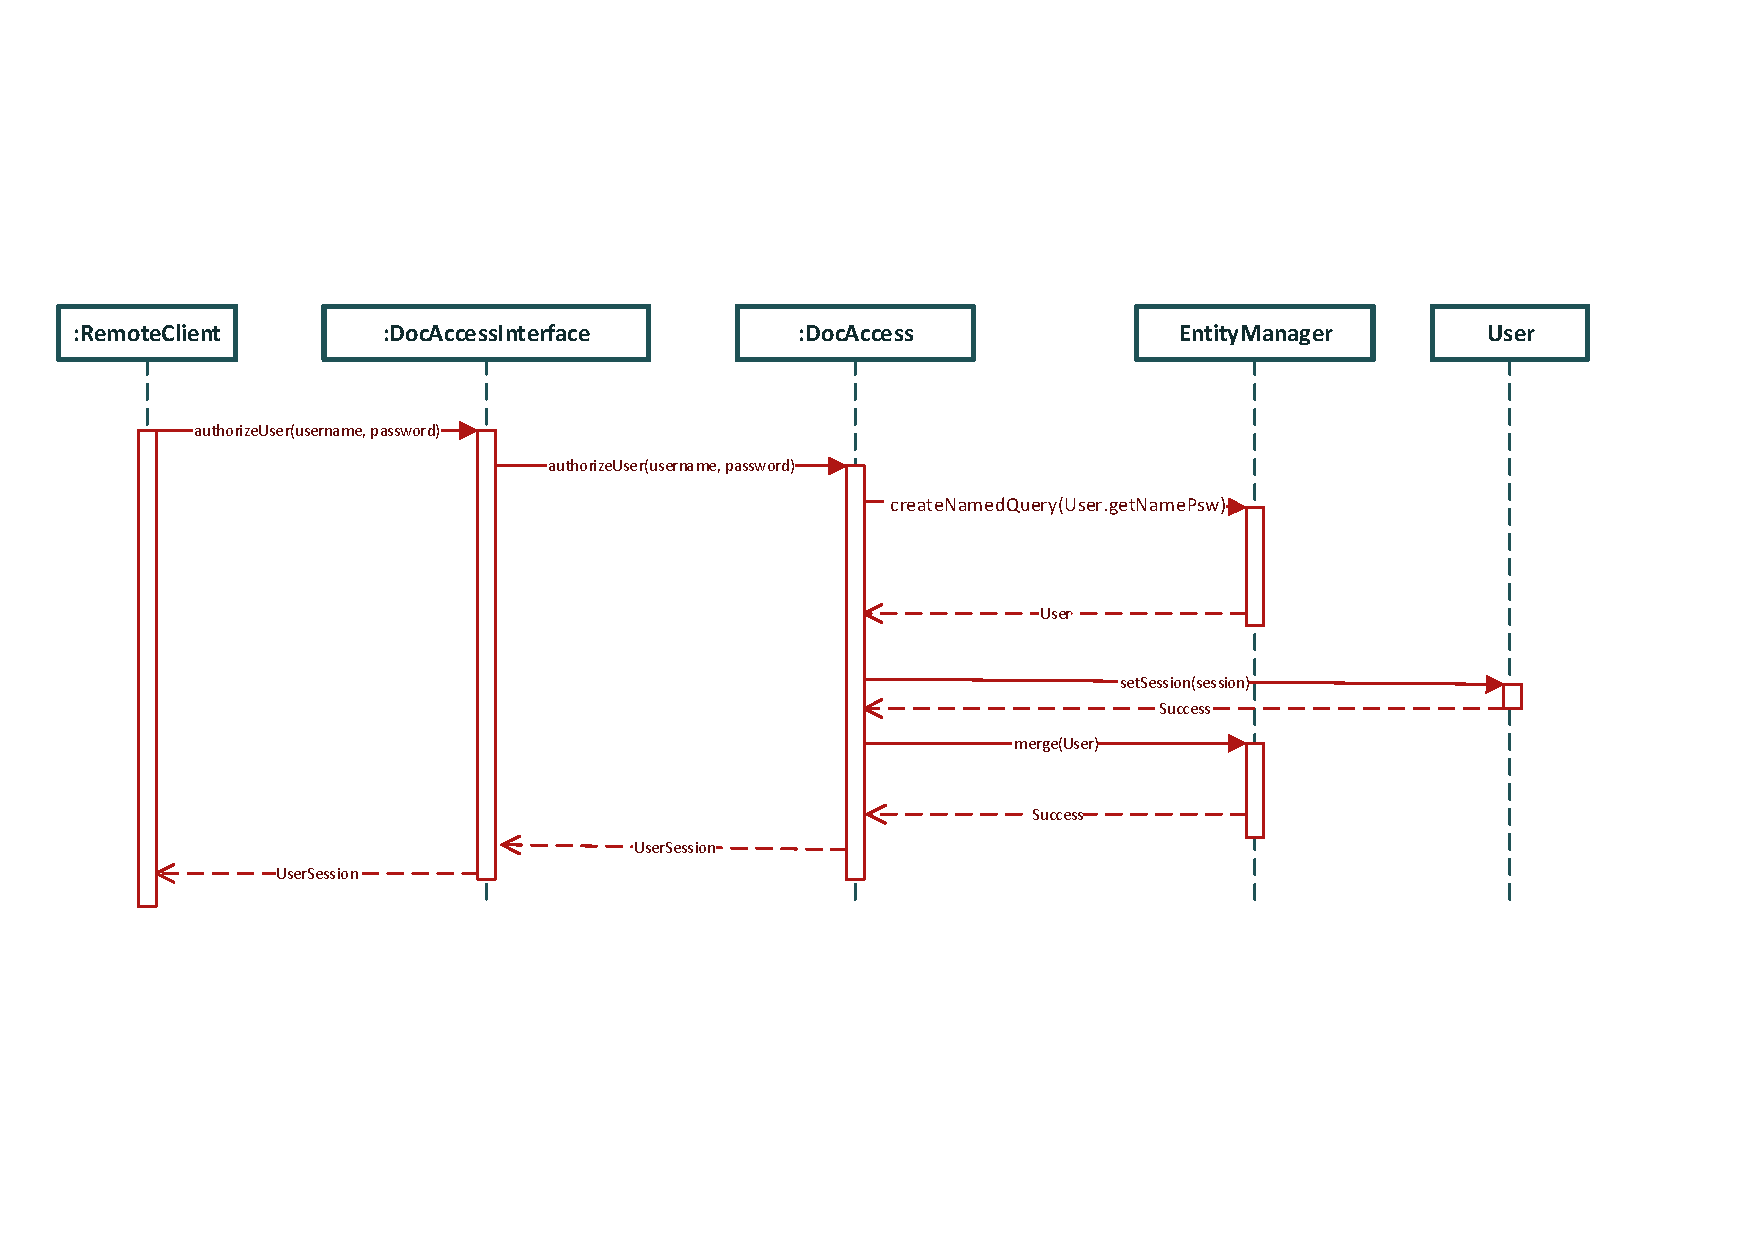
\includegraphics[width=1\textwidth]{login}
	\caption{Авторизация}
	\label{fig:login}
\end{figure}

\begin{figure}[H]
\centering
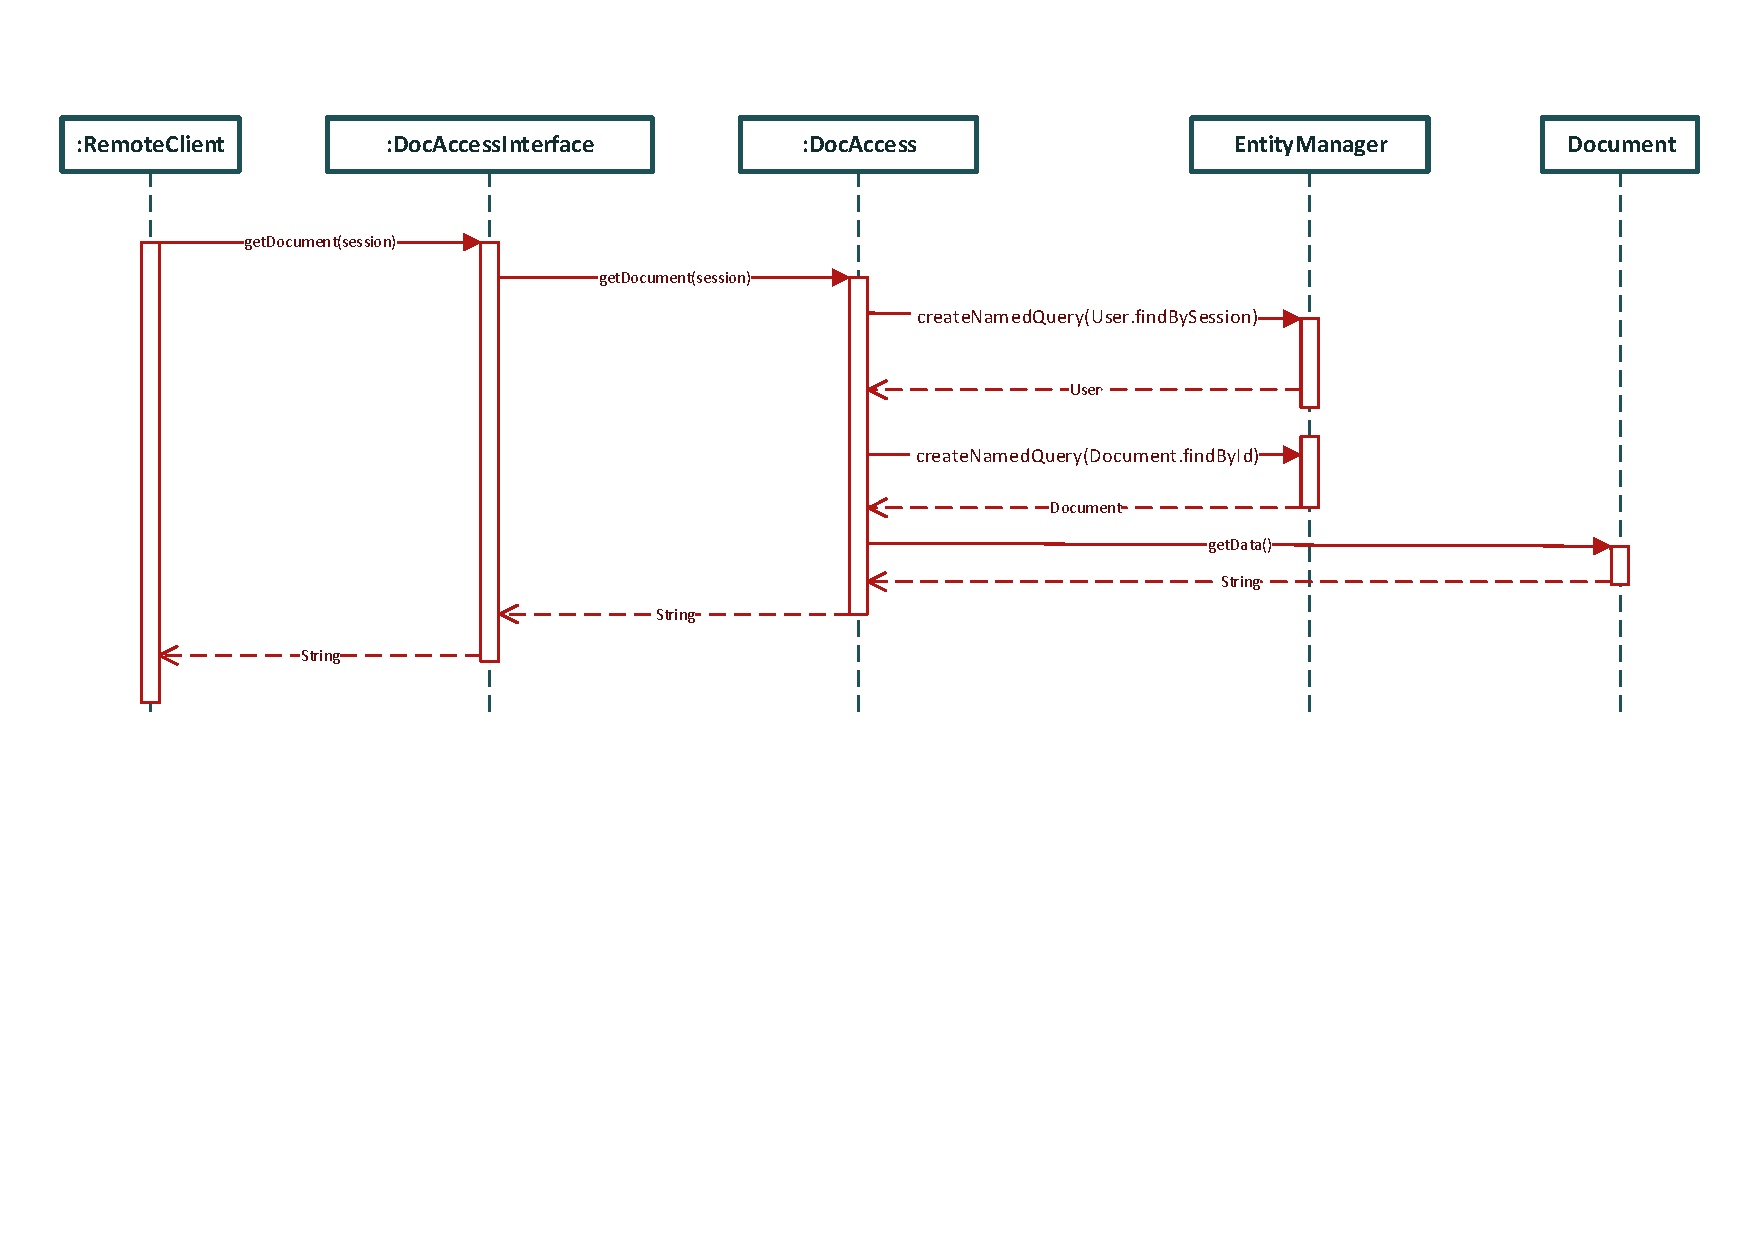
\includegraphics[width=1\textwidth]{getDoc}
\caption{Получение последней версии документа}
\label{fig:getdoc}
\end{figure}

\begin{figure}[H]
	\centering
	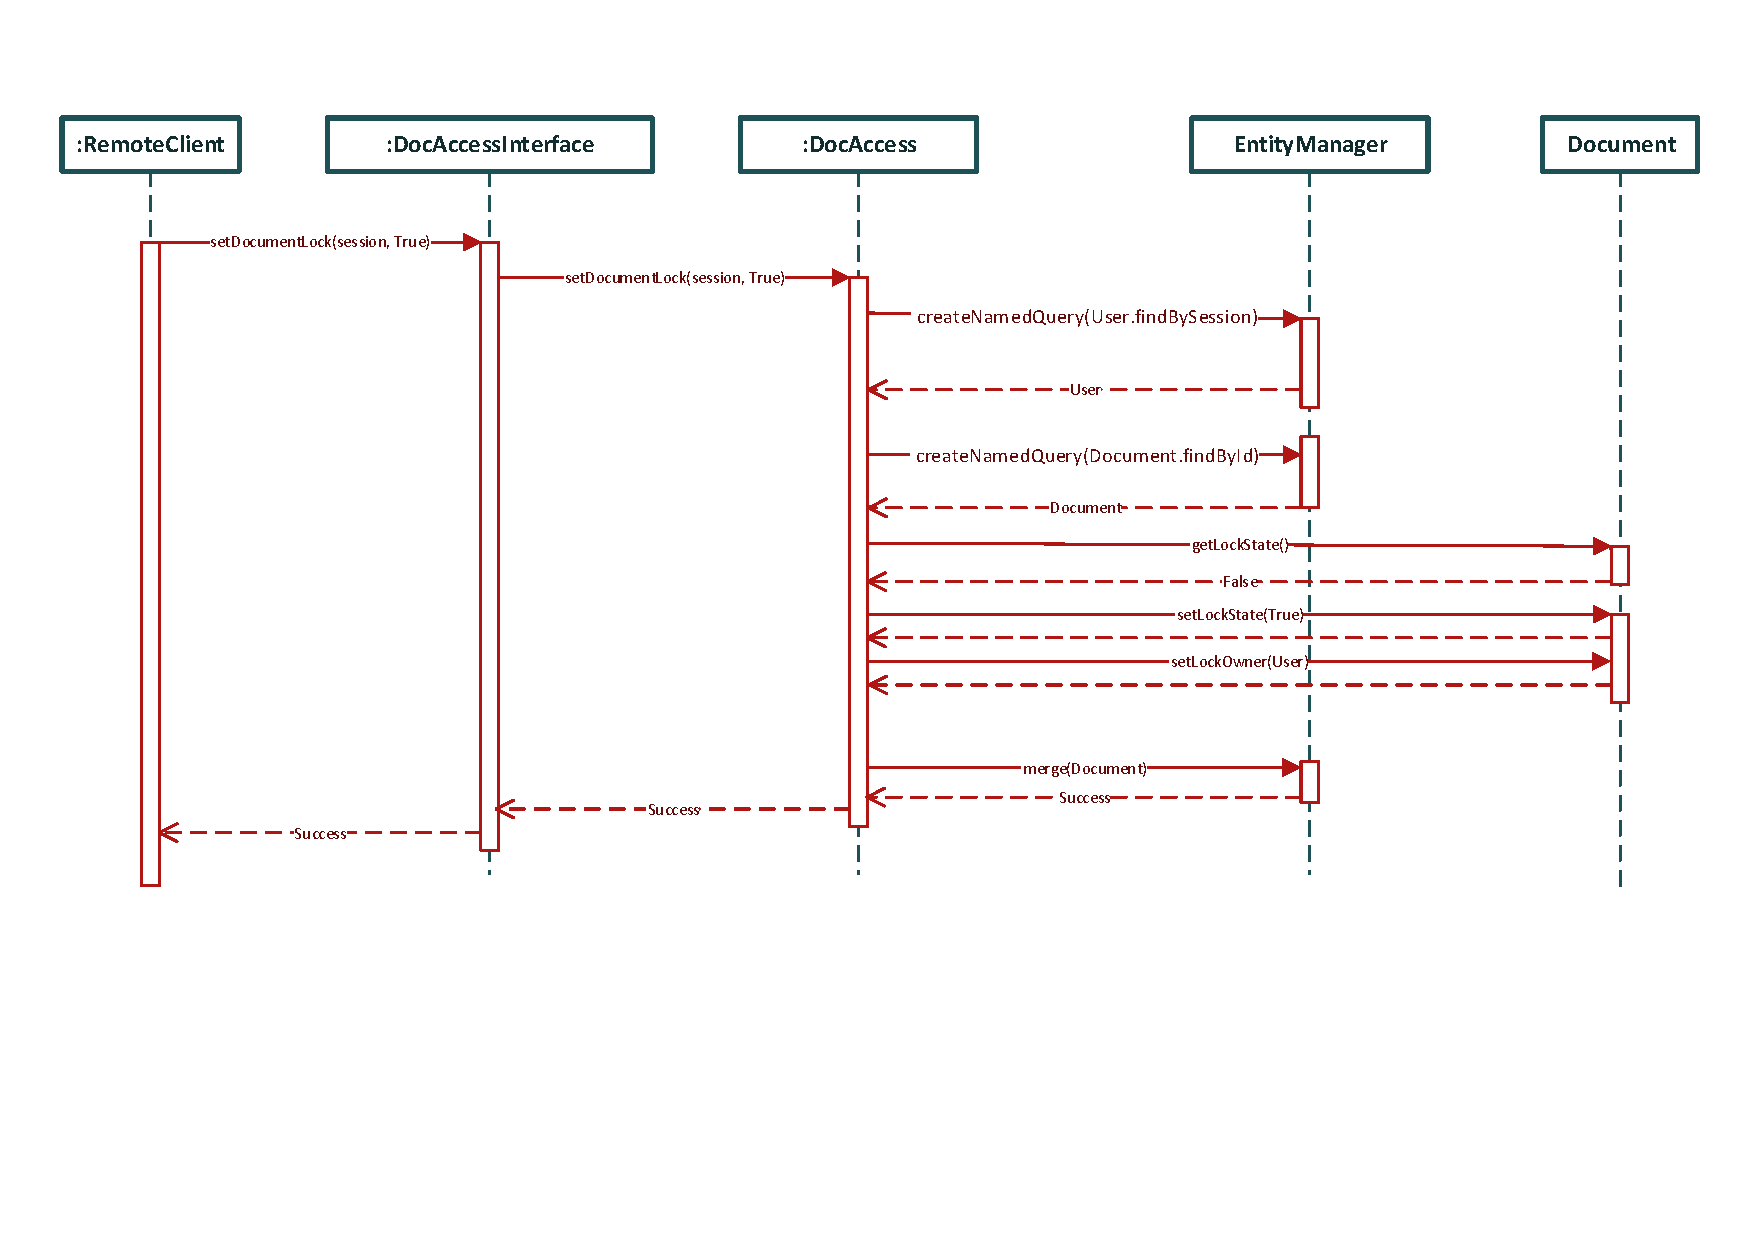
\includegraphics[width=1\textwidth]{setLockTrue}
	\caption{Получение эксклюзивного доступа}
	\label{fig:lock}
\end{figure}

\begin{figure}[H]
	\centering
	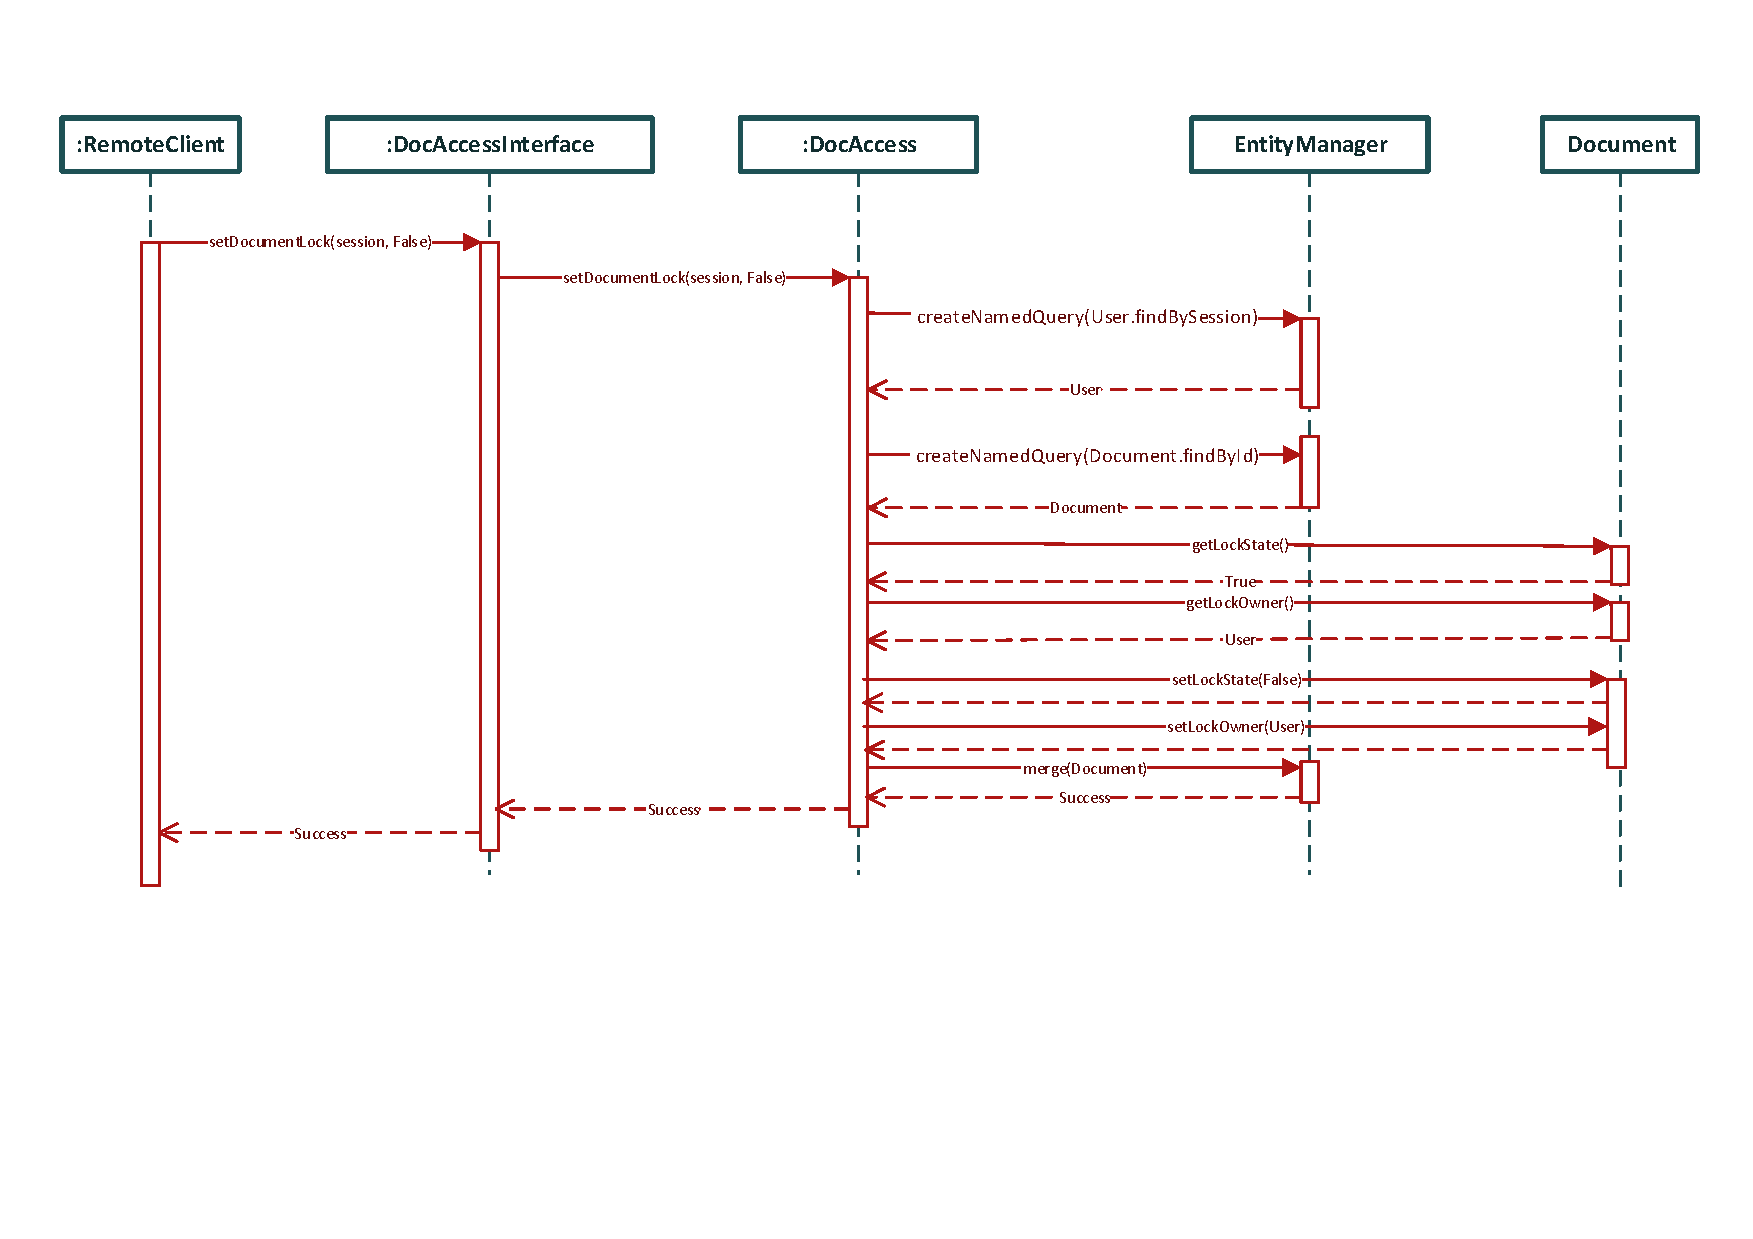
\includegraphics[width=1\textwidth]{setLockFalse}
	\caption{Снятие блокировки}
	\label{fig:unlock}
\end{figure}

\begin{figure}[H]
	\centering
	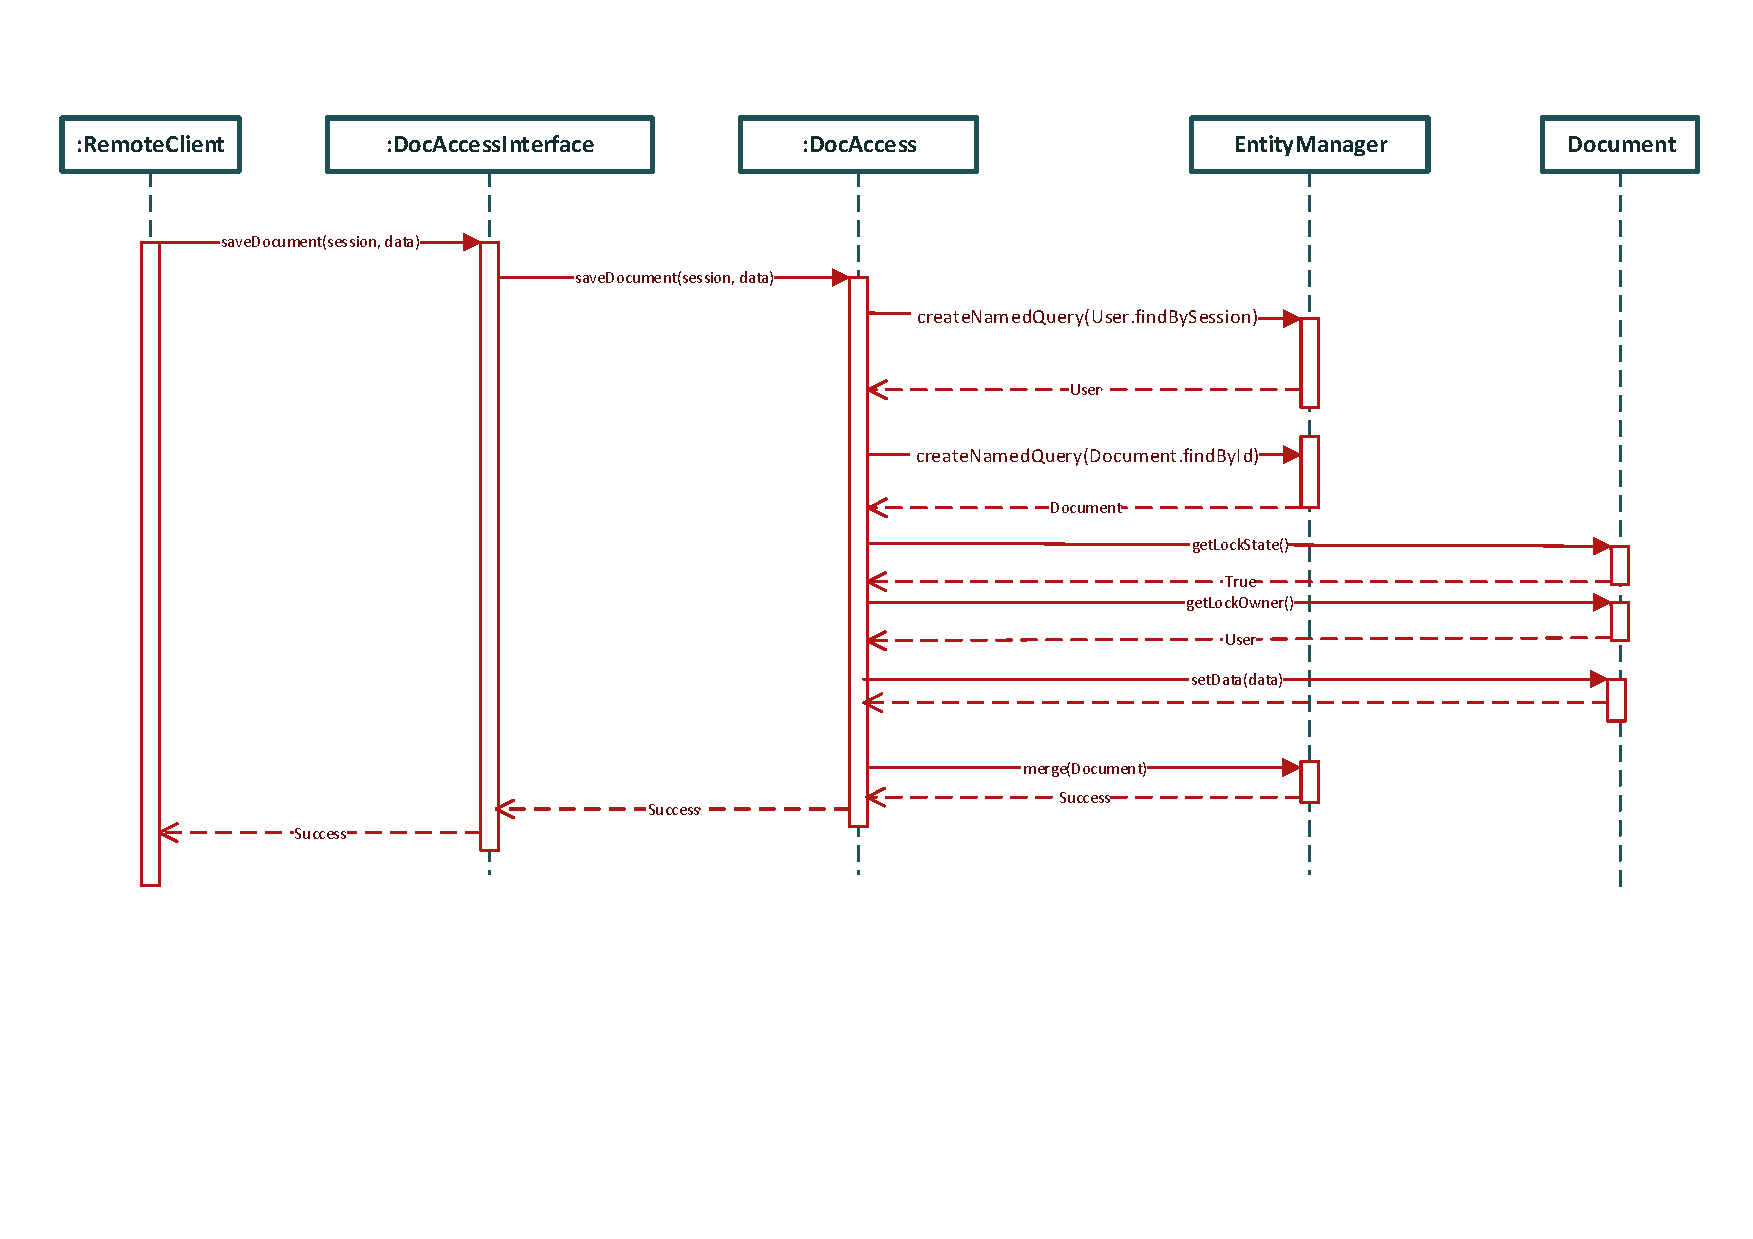
\includegraphics[width=1\textwidth]{saveDoc}
	\caption{Сохранение документа}
	\label{fig:save}
\end{figure}